%======================================================================
%----------------------------------------------------------------------
%               XX                              X
%                                               X
%               XX    XXX   XXX   XXX      XXX  X  XXXX
%                X   X   X X   X X   X    X   X X X
%                X   XXXXX XXXXX XXXXX    X     X  XXX
%                X   X     X     X     XX X   X X     X
%               XXX   XXX   XXX   XXX  XX  XXX  X XXXX
%----------------------------------------------------------------------
%  	         A SKELETON FILE FOR IEEE PAPER GENERATION
%----------------------------------------------------------------------
%    Modificado por: Edgardo Vaz, Melina Rabinovich, Daniel Aicardi.  
%                                     2011                            
%======================================================================

% first, uncomment the desired options:
\documentclass[%
        %draft,
        %submission,
        %compressed,
        final,
        %
        %technote,
        %internal,
        %submitted,
        %inpress,
        %reprint,
        %
        %titlepage,
        notitlepage,
        %anonymous,
        narroweqnarray,
        inline,
        %twoside,
        ]{ieee}
%
% some standard modes are:
%
% \documentclass[draft,narroweqnarray,inline]{ieee}
% \documentclass[submission,anonymous,narroweqnarray,inline]{ieee}
% \documentclass[final,narroweqnarray,inline]{ieee}

% Use the `endfloat' package to move figures and tables to the end
% of the paper. Useful for `submission' mode.
%\usepackage {endfloat}

% Use the `times' package to use Helvetica and Times-Roman fonts
% instead of the standard Computer Modern fonts. Useful for the 
% IEEE Computer Society transactions.
% (Note: If you have the commercial package `mathtime,' it is much
% better, but the `times' package works too).
%\usepackage {times}

% In order to use the figure-defining commands in ieeefig.sty...
\usepackage{ieeefig}
\usepackage[utf8]{inputenc}

\begin{document}

%----------------------------------------------------------------------
% Title Information, Abstract and Keywords
%----------------------------------------------------------------------
\title[Specification for Common IEEE Styles]{%
       Recarga Fácil por Radio Frecuencia, RF$^{2}$}

% format author this way for journal articles.
\author[SHORT NAMES]{%
	 Melina Rabinovich, Edgardo Vaz, Daniel Aicardi
	\thanks{M. Rabinovich, E. Vaz y  D. Aicardi Facultad de Ingeniería, Universidad de la República Oriental del Uruguay, Montevideo, Uruguay,
		{\tt\small mrabinovichm@gmail.com, edgardovaz@gmail.com, daicav@gmail.com} }
}


% specifiy the journal name
%\journal{IEEE Transactions on Something, 1997}

% Or, when the paper is a preprint, try this...
%\journal{IEEE Transactions on Something, 1997, TN\#9999.}

% Or, specify the conference place and date.
%\confplacedate{Ottawa, Canada, May 19--21, 1997}

% make the title
\maketitle               

% do the abstract
\begin{abstract}
El presente documento muestra las características de hardware y software que componen un prototipo de sistema embebido enfocado a operar con tarjetas RFID (ISO14443) como las que son utilizadas actualmente en el sistema de transporte de la ciudad de Montevideo.
\end{abstract}

\bigskip

% do the keywords
\begin{keywords}
Tarjetas inteligentes con y sin contacto, RFID, ISO14443, Mifare, CL RC632.
\end{keywords}

% start the main text ...
%----------------------------------------------------------------------
% SECTION I: Introduccion
%----------------------------------------------------------------------
\section{Introducción}

\PARstart El uso de tarjetas inteligentes es cada vez más frecuente en todos los ámbitos de nuestra vida cotidiana. 
Tal es el caso del sistema de transporte de la ciudad de Montevideo, donde cada pasajero utiliza una tarjeta RFID 
para efectuar el pago de cada viaje. Esto último implica que cada usuario debe cargar saldo en su tarjeta para su 
posterior uso. Es necesario entonces brindar un mecanismo simple, seguro y rápido que permita asignar saldo a cada tarjeta; la siguiente figura muestra un diagrama simplificado del sistema.

\begin{figure}[h]
\centering
  \begin{center}
  	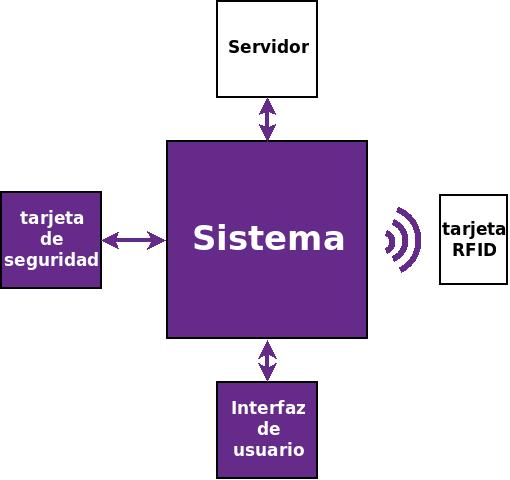
\includegraphics[scale=.3]{../pres_fin/Imagenes/diagrama_def.jpg} 
  	\caption{Bloques que conforman el sistema}\label{sist_gral} 
  \end{center}		 
\end{figure}

De los conceptos antes mencionados, se decidió implementar los bloques correspondientes al 
sistema que incluye el lector/escritor de tarjetas RFID, el lector/escritor de tarjetas 
de seguridad y la interfaz de usuario.
No fueron implementados los bloques relativos al servidor y las tarjetas RFID.

\bigskip
Las partes implementadas forman un prototipo de sistema embebido que interactúa con tarjetas RFID,
permitiendo consultar y/o acreditar saldo en las mismas.
El mecanismo de transferir saldo en las tarjetas RFID mediante éste dispositivo, se encuentra
desacoplado del sistema de pago de dinero, el cual podría efectuarse a través de una red de pagos,
mensajes de texto, web, etc, esto último no forma parte de este proyecto por tanto no fue implementado.


\bigskip
%----------------------------------------------------------------------
% SECTION II: Objetivo
%----------------------------------------------------------------------
\section{Objetivo}
El objetivo del proyecto es la fabricación de un prototipo de sistema embebido capaz de consultar y recargar tarjetas. Para ésto, como se mencionó en la introducción, deberá lograr establecer comunicación con tarjetas  como las utilizadas en el Sistema de Transporte Metropolitano (comunicación RFID a 13,56 MHz), con tarjetas de contacto (módulo de seguridad SAM), y con el usuario a través de una interfaz simple.

\bigskip
Esto implica entonces la fabricación de dos lectores/escritores de tarjetas, uno para tarjetas RFID (sin contacto) y
otro para tarjetas con contacto (SAM), una interfaz para el usuario capaz de informar el estado de la transacción
mediante mensajes adecuados, y la utilización de un sistema basado en un microprocesador para controlar los periféricos
y realizar las operaciones. Esto último implica además el desarrollo del software para que todo funcione adecuadamente.


\bigskip
%----------------------------------------------------------------------
% SECTION III: Hardware
%----------------------------------------------------------------------
\section{Hardware}


\bigskip
%----------------------------------------------------------------------
% SECTION IV: Software
%----------------------------------------------------------------------
\section{Software}


\bigskip
%----------------------------------------------------------------------
% SECTION V: Costos
%----------------------------------------------------------------------
\section{Costos}


\bigskip
%----------------------------------------------------------------------
% SECTION VI: Conclusiones
%----------------------------------------------------------------------
\section{Conclusiones}
El mundo de la tecnología RFID está poco explorado en nuestro país, éste 
tal vez sea el primer proyecto que incluye el diseño y fabricación de un 
lector/escritor RFID capaz de operar con tarjetas sin contacto en la banda de
frecuencia de 13,56 MHz.

El aporte realizado en este campo es tan solo una primera aproximación y aún 
queda mucho por hacer al respecto. Sobre este proyecto en particular es
necesario mejorar varios aspectos antes de pasar de la fase de prototipo
a la de producción.

\bigskip
Repasando en particular los criterios de éxito, el proyecto ha resultado satisfactorio
porque se logró construir un dispositivo capaz de consultar y recargar tarjetas RFID,
aunque la solución alcanzada no sea estrictamente igual a la propuesta en el comienzo.


\bigskip
% do the biliography:
\bibliographystyle{IEEEbib}
\bibliography{my-bibliography-file}

% where ``my-bibliography-file.bib'' is the name of the file with all the 
% BibTeX entries.

% do the biographies...
%\begin{biography}{Autor}
%Aquí se detalla la biografía del autor.
%\end{biography}

% If you want a picture with your biography, then specify the name of
% the postscript file in square brackets. That is, uncomment the
% following three lines and change the name of "face.ps" to the name of 
% your file.
%\begin{biography}[face.ps]{Gregory L. Plett}
%  A bio with a face...
%\end{biography}

%----------------------------------------------------------------------
% FIGURES
%----------------------------------------------------------------------
% There are many ways to include figures in the text. We will assume
% that the figure is some sort of EPS file.
%
% The outdated packages epsfig and psfig allow you to insert figures
% like: \psfig{filename.eps} These should really be done now using the
% \includegraphics{filename.eps} command.  
%
% i.e.,
%
% \includegraphics{file.eps}
%
% whenever you want to include the EPS file 'file.eps'. There are many
% options for the includegraphics command, and are outlined in the
% on-line documentation for the "graphics bundle". Using the options,
% you can specify the height, total height (height+depth), width, scale,
% angle, origin, bounding box "bb",view port, and can trim from around
% the sides of the figure. You can also force LaTeX to clip the EPS file
% to the bounding box in the file. I find that I often use the scale,
% trim and clip commands.
% 
% \includegraphics[scale=0.6,trim=0 0 0 0,clip=]{file.eps}
% 
% which magnifies the graphics by 0.6 (If I create a graphics for an
% overhead projector transparency, I find that a magnification of 0.6
% makes it look much better in a paper), trims 0 points off
% of the left, bottom, right and top, and clips the graphics. If the
% trim numbers are negative, space is added around the figure. This can
% be useful to help center the graphics, if the EPS file bounding box is
% not quite right.
% 
% To center the graphics,
% 
% \begin{center}
% \includegraphics...
% \end{center}
% 
% I have not yet written good documentation for this, but another 
% package which helps in figure management is the package ieeefig.sty,
% available at: http://www-isl.stanford.edu/people/glp/ieee.shtml
% Specify:
% 
%\usepackage{ieeefig} 
% 
% in the preamble, and whenever you want a figure,
% 
%\figdef{filename}
% 
% where, filename.tex is a LaTeX file which defines what the figure is.
% It may be as simple as
% 
% \inserteps{filename.eps}
%
% or
% \inserteps[includegraphics options]{filename.eps}
% 
% or may be a very complicated LaTeX file. 

\end{document}
